\documentclass[10pt,aspectratio=169]{beamer}
\usetheme{Madrid}
\usecolortheme{seahorse}
\setbeamertemplate{navigation symbols}{}
\usepackage{graphicx}
\usepackage{booktabs}
\usepackage{amsmath}
\usepackage{tikz}
\usetikzlibrary{arrows.meta,positioning,calc}
\graphicspath{{../report/figs/}}
\newcommand{\um}{\,\mu\mathrm{m/ns}}

\title[Waveform-first reconstruction]{The waveform-first forward-fit reconstruction\\ for the MX17 micro-TPC}
\subtitle{threading solved $\cdot$ $v_\mathrm{drift}$ resolved $\cdot$ gas identified $\cdot$ in-situ gap maps}
\author{MX17 June cosmic-bench analysis}
\date{25--27 July 2026}

\begin{document}

\begin{frame}
\titlepage
\end{frame}

%----------------------------------------------------------------------
\begin{frame}{The starting problem: tracks don't ``thread'' the reference}
\begin{columns}
\column{0.55\textwidth}
\begin{itemize}\itemsep6pt
\item Micro-TPC: strip position + arrival time $\Rightarrow$ 3-D track per muon
\item Hit-level reconstruction: fitted ladders $\sim$4$^\circ$ \textbf{too steep};
the M3 reference threads the cloud at the mesh, fans away with depth
\item Not alignment ($<10\,\mu$m); ``unsharing'' fixed it only on average
\item \textbf{This work: rebuild from raw waveforms, zero assumptions}
\end{itemize}
\column{0.45\textwidth}
\centering
\includegraphics[width=\textwidth]{event_raw.png}\\
{\scriptsize one muon in the raw waveform matrix; dashed = M3 prediction}
\end{columns}
\end{frame}

%----------------------------------------------------------------------
\begin{frame}{How the micro-TPC works}
\centering
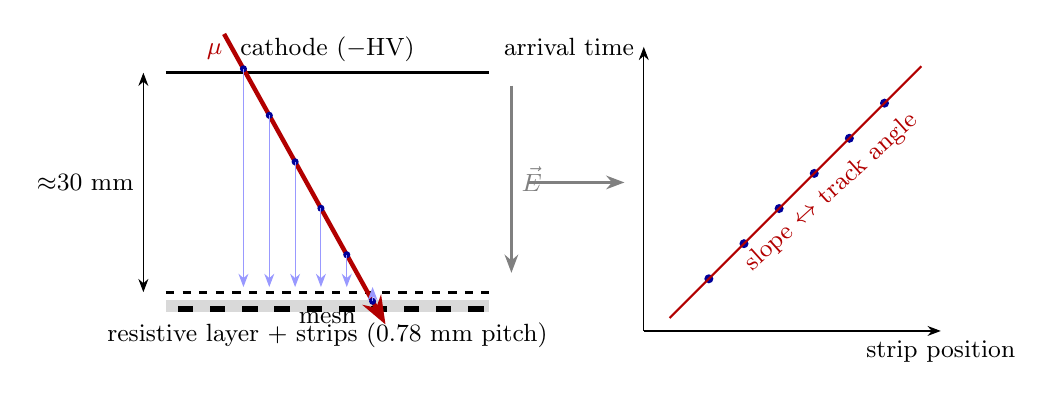
\begin{tikzpicture}[scale=0.82,>=Stealth]
\begin{scope}
  \draw[very thick] (0,4.0) -- (5,4.0) node[midway,above]{\small cathode ($-$HV)};
  \draw[very thick,dashed] (0,0.6) -- (5,0.6) node[midway,below,yshift=-1pt]{\small mesh};
  \fill[gray!30] (0,0.30) rectangle (5,0.48);
  \node[below] at (2.5,0.28) {\small resistive layer + strips (0.78 mm pitch)};
  \foreach \x in {0.3,0.8,...,4.8} \fill[black] (\x-0.12,0.30) rectangle (\x+0.12,0.38);
  \draw[->,thick,gray] (5.35,3.8) -- (5.35,0.9) node[midway,right]{\small $\vec E$};
  \draw[->,ultra thick,red!70!black] (0.9,4.6) -- (3.4,0.1) node[pos=0.06,left]{\small $\mu$};
  \foreach \t in {0.12,0.28,0.44,0.60,0.76,0.92} {
    \pgfmathsetmacro{\px}{0.9+2.5*\t}
    \pgfmathsetmacro{\py}{4.6-4.5*\t}
    \fill[blue!60!black] (\px,\py) circle (0.055);
    \draw[->,blue!40,thin] (\px,\py) -- (\px,0.68);
  }
  \draw[<->] (-0.35,0.6) -- (-0.35,4.0) node[midway,left]{\small $\approx$30 mm};
\end{scope}
\begin{scope}[xshift=7.4cm]
  \draw[->] (0,0) -- (4.6,0) node[below]{\small strip position};
  \draw[->] (0,0) -- (0,4.4) node[left]{\small arrival time};
  \foreach \t in {0.12,0.28,0.44,0.60,0.76,0.92} {
    \pgfmathsetmacro{\px}{0.6+3.4*\t}
    \pgfmathsetmacro{\py}{0.4+3.4*\t}
    \fill[blue!60!black] (\px,\py) circle (0.07);
  }
  \draw[red!70!black,thick] (0.4,0.2) -- (4.3,4.1);
  \node[red!70!black,rotate=42] at (2.9,2.15) {\small slope $\leftrightarrow$ track angle};
\end{scope}
\draw[->,thick,gray] (5.6,2.3) -- (7.1,2.3);
\end{tikzpicture}\\[2mm]
\emph{Arrival time encodes depth. A straight muon = a straight line in (position, time).}
\end{frame}

%----------------------------------------------------------------------
\begin{frame}{Why every hit-based timing fails: the sharing mixture}
\begin{columns}
\column{0.47\textwidth}
\begin{itemize}\itemsep5pt
\item The resistive layer sends each strip's signal to its neighbours:
\textbf{delayed} ($\tau_s\!\approx\!47$ ns) and \textbf{dispersed}
($\sigma_s\!\approx\!90$ ns), $c_1\!\approx\!29\%$ each side
\item Neighbours' charge arrived at \emph{different depths/times}
\item Any time extracted from the aggregate is pulled toward the cluster mean
\item Measured: $+40$ ns late at the mesh, $-100$ ns early at the cathode,
\textbf{same for every estimator} $\Rightarrow$ ladder compressed 20--30\%
$\Rightarrow$ ``4$^\circ$ too steep''
\end{itemize}
\column{0.53\textwidth}
\centering
\includegraphics[width=\textwidth]{estimator_residual_curves.png}
\end{columns}
\end{frame}

%----------------------------------------------------------------------
\begin{frame}{The fix: fit the waveforms, not the hits}
\centering
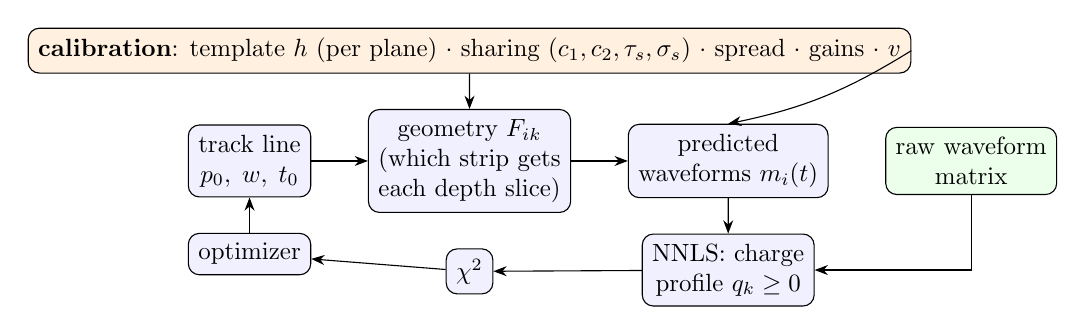
\begin{tikzpicture}[>=Stealth,node distance=4mm,scale=0.9, every node/.style={transform shape},
  box/.style={draw,rounded corners,align=center,fill=blue!6,inner sep=4pt},
  data/.style={draw,rounded corners,align=center,fill=green!8,inner sep=4pt},
  hyp/.style={draw,rounded corners,align=center,fill=orange!12,inner sep=4pt}]
\node[box] (par) {track line\\ $p_0,\; w,\; t_0$};
\node[box,right=8mm of par] (geo) {geometry $F_{ik}$\\ (which strip gets\\ each depth slice)};
\node[hyp,above=5mm of geo] (cal) {\textbf{calibration}: template $h$ (per plane) $\cdot$
sharing $(c_1,c_2,\tau_s,\sigma_s)$ $\cdot$ spread $\cdot$ gains $\cdot$ $v$};
\node[box,right=8mm of geo] (mat) {predicted\\ waveforms $m_i(t)$};
\node[data,right=8mm of mat] (dat) {raw waveform\\ matrix};
\node[box,below=5mm of mat] (nnls) {NNLS: charge\\ profile $q_k\ge0$};
\node[box,below=5mm of geo] (chi) {$\chi^2$};
\node[box,below=5mm of par] (opt) {optimizer};
\draw[->] (par) -- (geo); \draw[->] (geo) -- (mat); \draw[->] (cal) -- (geo);
\draw[->] (cal.east) to[bend left=10] (mat.north);
\draw[->] (mat) -- (nnls); \draw[->] (dat) |- (nnls);
\draw[->] (nnls) -- (chi); \draw[->] (chi) -- (opt); \draw[->] (opt) -- (par);
\end{tikzpicture}\\[1mm]
\small $m_i(t)=\sum_k q_k\big[F_{ik}h(t{-}t_0{-}u_k) + c_1(F_{i\pm1,k})h_s(t{-}t_0{-}u_k{-}\tau_s)+\ldots\big]$\\[1mm]
\begin{itemize}
\item Sharing modelled \textbf{forward} (well-conditioned) --- never deconvolved
\item Linear in the charges (fast NNLS); 3 nonlinear track parameters; $\sim$0.1 s/plane
\item $w=v\tan\theta$ in mm/ns: \textbf{no drift velocity assumed in the fit}
\end{itemize}
\end{frame}

%----------------------------------------------------------------------
\begin{frame}{Ingredients are measured, per detector}
\begin{columns}
\column{0.55\textwidth}
\centering
\includegraphics[width=\textwidth]{templates_perplane.png}\\
{\scriptsize impulse template from bright steep-track strips; Y undershoot 4$\times$ deeper}
\column{0.45\textwidth}
\textbf{Calibration protocol (automated):}
\begin{enumerate}\itemsep4pt
\item template per plane (data-driven)
\item gain map (det3: 1.4\% spread only)
\item 8-parameter hyper-fit with track pinned to M3 on $\sim$150 muons\\
{\small $(c_1,c_2,k_Y,\tau_s,\sigma_s,\sigma_{p0},D_p,v)$}
\end{enumerate}
\vspace{2mm}
{\small Anti-circularity: calibrating against the biased ladders instead is
49\% worse in $\chi^2$ --- the waveforms \emph{prefer} the reference tracks.}
\end{columns}
\end{frame}

%----------------------------------------------------------------------
\begin{frame}{One event, fitted}
\centering
\includegraphics[width=0.95\textwidth]{event_fit.png}\\
{\small data $\cdot$ model $\cdot$ residual; fitted $10.9^\circ$ vs M3 $10.4^\circ$}
\end{frame}

%----------------------------------------------------------------------
\begin{frame}{Performance: head-to-head on identical events}
\begin{columns}
\column{0.58\textwidth}
\centering
\includegraphics[width=\textwidth]{three_way_comparison.png}
\column{0.42\textwidth}
\small
\begin{tabular}{lcc}
\toprule
 & angle $\sigma$ & $<$1mm depth\\
\midrule
raw ladder & $5.0/5.7^\circ$ & 24/16\%\\
SOTA hybrid & $1.6/1.5^\circ$ & ---\\
\textbf{forward fit} & $\mathbf{1.06/1.10^\circ}$ & \textbf{74/70\%}\\
\bottomrule
\end{tabular}
\vspace{3mm}
\begin{itemize}\itemsep4pt
\item mesh position $\sigma$ = 0.57/0.59 mm
\item unbiased ($<0.3^\circ$), flat implied-$v$ vs angle (physical)
\item all angles: $\sim$1.0--1.1$^\circ$ for $|\tan\theta|>0.04$
\end{itemize}
\end{columns}
\end{frame}

%----------------------------------------------------------------------
\begin{frame}{The remaining $1^\circ$ is physics, not reconstruction}
\centering
\small
\begin{tabular}{lcc}
\toprule
toy truth & angle $\sigma$ recovered & $p_0$ $\sigma$\\
\midrule
electronics noise only & $\mathbf{0.02^\circ}$ & 7 $\mu$m\\
+0.15 mm/bin charge-centroid jitter & $0.55^\circ$ & 219 $\mu$m\\
\textbf{+0.30 mm/bin (diffusion scale)} & $\mathbf{1.05^\circ}$ & 354 $\mu$m\\
+0.50 mm/bin & $1.77^\circ$ & 473 $\mu$m\\
\bottomrule
\end{tabular}
\vspace{4mm}
\begin{itemize}\itemsep5pt
\item Toy closure: model-generated waveforms with known tracks, real noise/geometry
\item The observed $1.05^\circ$ = \textbf{stochastic diffusion + avalanche-weighted
charge granularity} --- the detector's information limit
\item Ablations: no single model component moves the width by $>0.05^\circ$
$\Rightarrow$ a production implementation can stay simple
\end{itemize}
\end{frame}

%----------------------------------------------------------------------
\begin{frame}{The drift-velocity tension: resolved}
\centering
\includegraphics[width=0.8\textwidth]{vtension_resolution.png}\\
{\small $v(1000\,\mathrm{V}) = 36.7 \pm 0.3\,(\mathrm{fit}) \pm 0.9\,(\mathrm{model})\um$;
the geometric 34.3 was a 1.3 mm spatial-floor-subtraction bias}
\end{frame}

%----------------------------------------------------------------------
\begin{frame}{The gas, identified by Magboltz}
\begin{columns}
\column{0.58\textwidth}
\centering
\includegraphics[width=\textwidth]{v_vs_E_forward_refined.png}
\column{0.42\textwidth}
\centering
\includegraphics[width=\textwidth]{rms_vs_h2o.png}\\
\vspace{2mm}
\small
\begin{itemize}\itemsep4pt
\item 71 mixtures (41 new: local + condor; cross-validated to 0.01$\um$)
\item \textbf{Ar/iC$_4$H$_{10}$ 95/5 + 0.8\% H$_2$O}, RMS 0.63$\um$ ($\ge$700 V)
\item consistent with the week's bottle drying
\end{itemize}
\end{columns}
\end{frame}

%----------------------------------------------------------------------
\begin{frame}{A scare that became a measurement: the drift-gap maps}
\begin{columns}
\column{0.5\textwidth}
\small
\textbf{The deconvolved charge profile's endpoint} $U$ measures the local gap:
$g = v\cdot U$.
\begin{itemize}\itemsep4pt
\item first pass said 24.7 mm (!) --- traced to two estimator biases
(median over sparse NNLS; free-fit profiles)
\item corrected: $U_{50}=762$ ns $\Rightarrow$ \textbf{27.9 mm}, stable vs
basis length, \textbf{closure-validated} (toys recover known columns to
$\le$5 ns, even with wrong-undershoot generation)
\item the edge is \emph{soft} where toy steps are sharp $\Rightarrow$
\textbf{the gap varies with position}
\end{itemize}
\column{0.5\textwidth}
\centering
\includegraphics[width=\textwidth]{K_scan.png}
\end{columns}
\end{frame}

%----------------------------------------------------------------------
\begin{frame}{det3's cathode is tilted; det4 bowed; det2 flat}
\centering
\includegraphics[width=0.8\textwidth]{gap_map.png}\\[1mm]
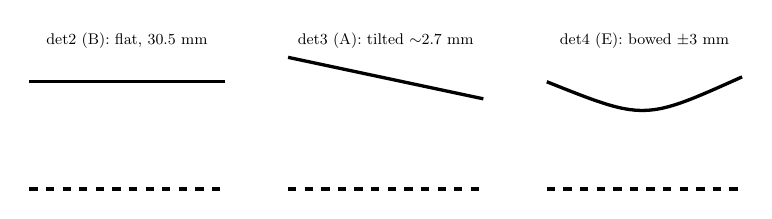
\begin{tikzpicture}[scale=0.62,>=Stealth, every node/.style={transform shape}]
\foreach \i/\name/\tilta/\tiltb in {0/{det2 (B): flat, 30.5 mm}/0/0,
                                    1/{det3 (A): tilted $\sim$2.7 mm}/0.5/-0.35,
                                    2/{det4 (E): bowed $\pm$3 mm}/0/0} {
 \begin{scope}[xshift=5.3cm*\i]
  \draw[very thick,dashed] (0,0) -- (4,0);
  \ifnum\i=2
    \draw[very thick] (0,2.2) .. controls (2,1.4) .. (4,2.3);
  \else
    \draw[very thick] (0,2.2+\tilta) -- (4,2.2+\tiltb);
  \fi
  \node[above] at (2,2.75) {\small \name};
 \end{scope}
}
\end{tikzpicture}\\
{\small mild $E^2$ electrostatic pull on top (28.4$\to$27.8 mm, 900$\to$1100 V).
\textbf{No short gap; no disassembly required} --- $U_{50}(x,y)$ is a free in-situ
flatness survey per chamber.}
\end{frame}

%----------------------------------------------------------------------
\begin{frame}{The production stack, validated on three chambers}
\centering
\small
\begin{tabular}{lccc}
\toprule
 & det3 (A) & det2 (B) & det4 (E)\\
\midrule
kernel $c_1$/$k_Y$/$\tau_s$ & 0.29/1.38/47 ns & 0.29/1.42/49 ns & 0.24/2.36/68 ns\\
$v$ (run conditions) & 36.6$\um$ & 39.9$\um$ & 34.2$\um$\\
angle $\sigma$ (x/y) & $1.06/1.10^\circ$ & $1.33/1.54^\circ$ & $2.00/1.97^\circ$\\
mesh $\sigma$ (x/y) & 0.57/0.59 mm & 0.76/0.56 mm & 0.93/0.71 mm\\
column / topography & 27.9 mm, y-tilt & 30.5 mm, \textbf{flat} & 28.8 mm, bowed\\
\bottomrule
\end{tabular}
\vspace{4mm}
\begin{itemize}\itemsep4pt
\item \texttt{wft\_reco.py}: \texttt{fit\_event()} $\to$ position, angle, charge profile,
honest errors (stat $\oplus$ physics floor), quality flags, near-vertical fallback
\item calibration scripts fully automated; handles different DAQ windows
\item plus: $\chi^2(v)$ gas monitor, gap mapper, cheap monitoring pre-pass
\end{itemize}
\end{frame}

%----------------------------------------------------------------------
\begin{frame}{Conclusions}
\begin{itemize}\itemsep8pt
\item \textbf{Threading solved}: the divergence was aggregate-time mixing from
resistive sharing; the forward fit removes it per event
\item \textbf{$\sigma\approx1^\circ$ / 0.6 mm per event --- at the physics floor}
(diffusion + charge granularity; noise contributes $0.02^\circ$)
\item \textbf{$v_\mathrm{drift}=36.7\pm0.3\pm0.9\um$}; gas = wet 95/5
(0.8\% H$_2$O), Magboltz-matched across the full drift scan
\item \textbf{Drift-gap topography measured in situ}: det3 tilted 2.7 mm,
det4 bowed, det2 flat at 30.5 mm
\item \textbf{Next}: mechanical flatness check at next opening; humidity probe;
300/500 V re-scan; det6/7; numba port; July beam data
\end{itemize}
\vspace{3mm}
\centering\small
\emph{Report: \texttt{waveform\_first\_threading/report/main.pdf} $\cdot$
full trail: \texttt{WAVEFORM\_FIRST\_THREADING.md} $\cdot$ scripts 01--36}
\end{frame}

\end{document}
